\documentclass{beamer}

\usepackage[outputdir=build]{minted}
\usepackage[spanish]{babel}
\graphicspath{ {../img/} {../../LaTeX/img/} {/home/csp98/latex/img/}}
\selectlanguage{spanish}
\newtheorem{ppio_invarianza}{Principio de Invarianza}
\usepackage[utf8]{inputenc}

%\usetheme{AnnArbor}
%\usetheme{Antibes}
%\usetheme{Bergen}
%\usetheme{Berkeley}
%\usetheme{Berlin}
%\usetheme{Boadilla}
%\usetheme{boxes}
%\usetheme{CambridgeUS}
%\usetheme{Copenhagen}
%\usetheme{Darmstadt}
%\usetheme{default}
%\usetheme{Frankfurt}
%\usetheme{Goettingen}
%\usetheme{Hannover}
%\usetheme{Ilmenau}
%\usetheme{JuanLesPins}
%\usetheme{Luebeck}
%\usetheme{Madrid}
%\usetheme{Malmoe}
%\usetheme{Marburg}
%\usetheme{Montpellier}
\usetheme{PaloAlto}
%\usetheme{Pittsburgh}
%\usetheme{Rochester}
%\usetheme{Singapore}
%\usetheme{Szeged}
%\usetheme{Warsaw}

\title{Práctica 1}

% A subtitle is optional and this may be deleted
\subtitle{Análisis de eficiencia de algoritmos}

\author{María Jesús López Salmerón \\ Nazaret Román Guerrero \\ Laura Hernández Muñoz \\ José Baena Cobos  \\ Carlos Sánchez Páez}


\makeatletter
  \setbeamertemplate{sidebar \beamer@sidebarside}%{sidebar theme}
  {
    \beamer@tempdim=\beamer@sidebarwidth%
    \advance\beamer@tempdim by -6pt%
    \insertverticalnavigation{\beamer@sidebarwidth}%
    \vfill
    \ifx\beamer@sidebarside\beamer@lefttext%
    \else%
      \usebeamercolor{normal text}%
      \llap{\usebeamertemplate***{navigation symbols}\hskip0.1cm}%
      \vskip2pt%
    \fi%
}%
\makeatother

\subject{Algorítmica}
% This is only inserted into the PDF information catalog. Can be left
% out. 

% If you have a file called "university-logo-filename.xxx", where xxx
% is a graphic format that can be processed by latex or pdflatex,
% resp., then you can add a logo as follows:

% \pgfdeclareimage[height=0.5cm]{university-logo}{university-logo-filename}
% \logo{\pgfuseimage{university-logo}}

% Delete this, if you do not want the table of contents to pop up at
% the beginning of each subsection:
\AtBeginSubsection[]
{
  \begin{frame}<beamer>{Índice}
    \tableofcontents[currentsection,currentsubsection]
  \end{frame}
}

% Let's get started
\begin{document}

\begin{frame}
  \titlepage
\end{frame}

\begin{frame}{Índice}
  \tableofcontents
  % You might wish to add the option [pausesections]
\end{frame}

% Section and subsections will appear in the presentation overview
% and table of contents.
\section{Cálculo de la eficiencia empírica}

\subsection{Diseño de scripts}

\begin{frame}[fragile]{Script individual}

\begin{minted}[fontsize=\small]{bash}
	#!/bin/bash
	if [ $# -eq 3 ]
	then
		i="0"
		output="out"
		tam=$2
		#Primer argumento: programa a ejecutar
		#Segundo argumento: tamaño inicial
		#Tercer argumento : incremento
		while [ $i -lt 25 ]
		do
			./$1 $tam >> $1.out
			i=$[$i+1]
			tam=$[$tam+$3]
		done
	else
		echo "Error de argumentos"
	fi
\end{minted}  
\end{frame}

\begin{frame}[fragile]{Script conjunto}

\begin{minted}[fontsize=\small]{bash}
	#!/bin/bash
	echo "Ejecutando burbuja..."
	./individual.sh burbuja 1000 1000
	echo "Ejecutando insercion..."
	./individual.sh insercion 1000 1000
	echo "Ejecutando seleccion..."
	./individual.sh seleccion 1000 1000
	echo "Ejecutando mergesort..."
	./individual.sh mergesort 1000000 500000
	echo "Ejecutando quicksort..."
	./individual.sh quicksort 1000000 500000
	echo "Ejecutando heapsort..."
	./individual.sh heapsort 1000000 500000
	echo "Ejecutando hanoi..."
	./individual.sh hanoi 10 1
	echo "Ejecutando floyd..."
	./individual.sh floyd 100 100
\end{minted}  
\end{frame}

\begin{frame}[fragile]{Makefile}

\begin{minted}[fontsize=\tiny]{makefile}
	DOC=doc
	SRC=src
	OUT=out
	BIN=src

	all : todos
	todos : burbuja floyd hanoi heapsort insercion mergesort quicksort seleccion
		cd $(SRC) ; ./todos.sh
	burbuja : 
		g++ -o ./$(BIN)/burbuja ./$(SRC)/burbuja.cpp
	floyd : 
		g++ -o ./$(BIN)/floyd ./$(SRC)/floyd.cpp
	hanoi : 
		g++ -o ./$(BIN)/hanoi ./$(SRC)/hanoi.cpp
	heapsort : 
		g++ -o ./$(BIN)/heapsort ./$(SRC)/heapsort.cpp
	insercion : 
		g++ -o ./$(BIN)/insercion ./$(SRC)/insercion.cpp
	mergesort : 
		g++ -o ./$(BIN)/mergesort ./$(SRC)/mergesort.cpp
	quicksort : 
		g++ -o ./$(BIN)/quicksort ./$(SRC)/quicksort.cpp
	seleccion :
		g++ -o ./$(BIN)/seleccion ./$(SRC)/seleccion.cpp
\end{minted}  
\end{frame}


\subsection{Modificación de código fuente}

\begin{frame}[fragile]{Modificación de código fuente}
\begin{minted}{c++}
	clock_t tantes;
	clock_t tdespues;
	tantes = clock();
	algoritmo_en_cuestion(T, n);
	tdespues = clock();
	cout << ((double)(tdespues - tantes))
	/ CLOCKS_PER_SEC << endl;
\end{minted}
\end{frame}

\subsection{Entornos de pruebas}

\subsection{Tamaños de problema}
\begin{frame}[fragile]{Tamaños de problema}
\begin{table}[H]
\centering
\begin{tabular}{|c|c|c|c|}
\hline
\textbf{Algoritmo} & \textbf{Eficiencia} & \textbf{Tamaño inicial} & \textbf{Incremento}\\
\hline
Burbuja & $O(n^2)$ & 1000 & 1000 \\
\hline
Inserción & $O(n^2)$ & 1000 & 1000 \\
\hline
Selección & $O(n^2)$ & 1000 & 1000 \\
\hline
Mergesort & $O(n \cdot log(n))$ & 1.000.000 & 500.000 \\
\hline
Quicksort & $O(n \cdot log(n))$ & 1.000.000 & 500.000 \\
\hline
Heapsort & $O(n \cdot log(n))$ & 1.000.000 & 500.000 \\
\hline
Floyd & $O(n^3)$ & 100 & 100 \\
\hline
Hanoi & $O(2^n)$ & 10 & 1 \\
\hline
\end{tabular}
\end{table}
\end{frame}
\subsection{Resultados}

\subsubsection{Algoritmos con eficiencia $O(n^2)$}

\begin{frame}[fragile]{Algoritmo burbuja}
\begin{figure}[H]
\centering
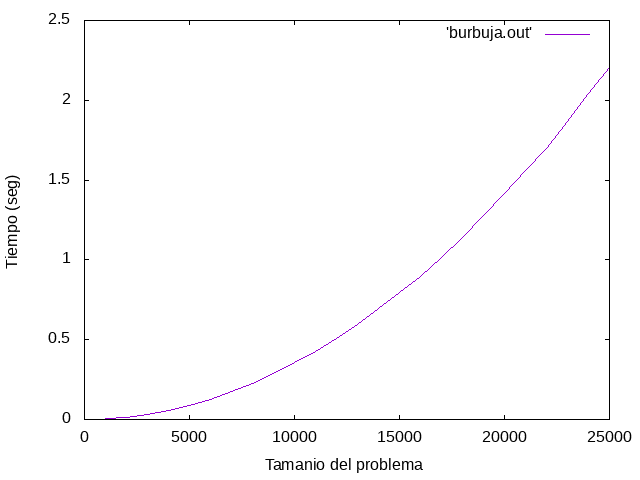
\includegraphics[scale=0.5]{empirica_burbuja.png}
\end{figure}
\end{frame}

\begin{frame}[fragile]{Algoritmo de inserción}
\begin{figure}[H]
\centering
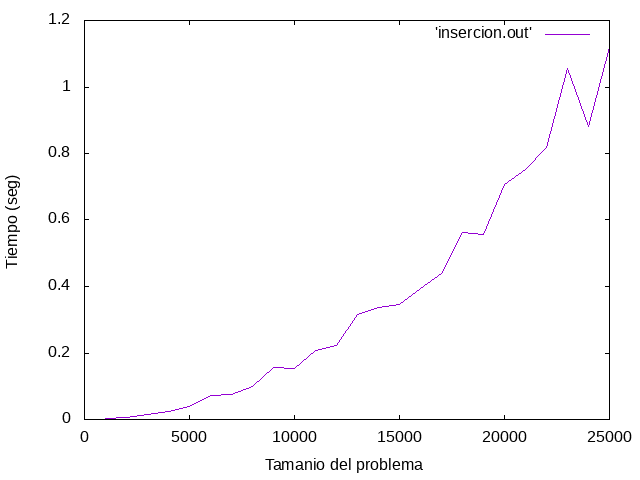
\includegraphics[scale=0.5]{empirica_insercion.png}
\end{figure}
\end{frame}

\begin{frame}[fragile]{Algoritmo de selección}
\begin{figure}[H]
\centering
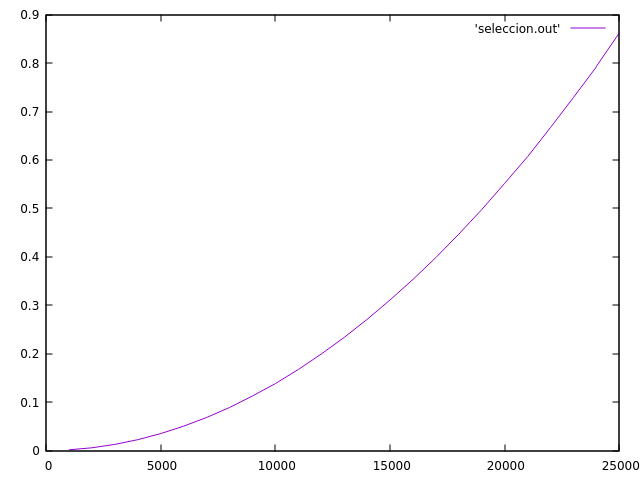
\includegraphics[scale=0.5]{empirica_seleccion.png}
\end{figure}
\end{frame}

\subsubsection{Algoritmo con eficiencia $O(n^3)$}
\begin{frame}[fragile]{Algoritmo de Floyd}
\begin{figure}[H]
\centering
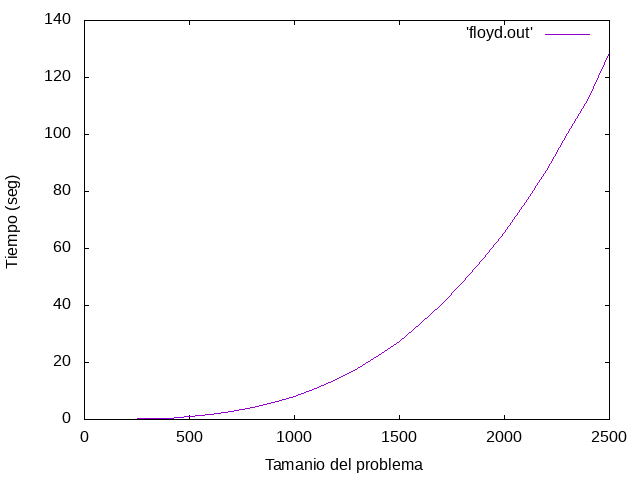
\includegraphics[scale=0.5]{empirica_floyd.png}
\end{figure}
\end{frame}

\subsubsection{Algoritmos con eficiencia $O(n \cdot log(n))$}

\begin{frame}[fragile]{Algoritmo mergesort}
\begin{figure}[H]
\centering
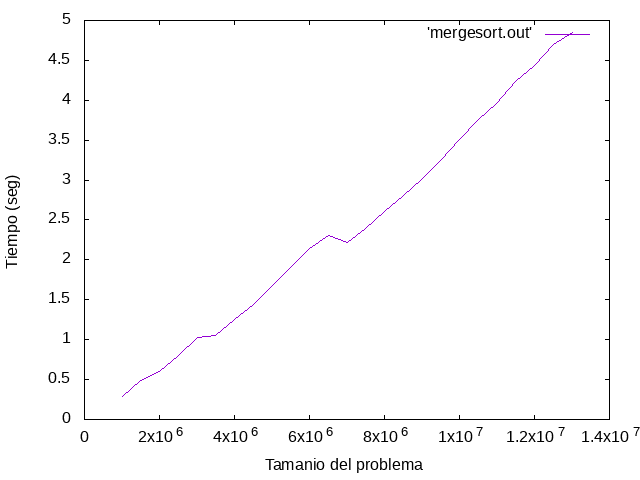
\includegraphics[scale=0.5]{empirica_mergesort.png}
\end{figure}
\end{frame}

\begin{frame}[fragile]{Algoritmo quicksort}
\begin{figure}[H]
\centering
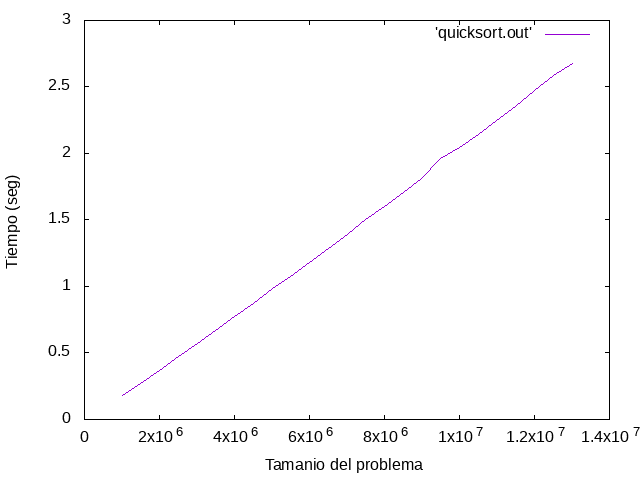
\includegraphics[scale=0.5]{empirica_quicksort.png}
\end{figure}
\end{frame}

\begin{frame}[fragile]{Algoritmo heapsort}
\begin{figure}[H]
\centering
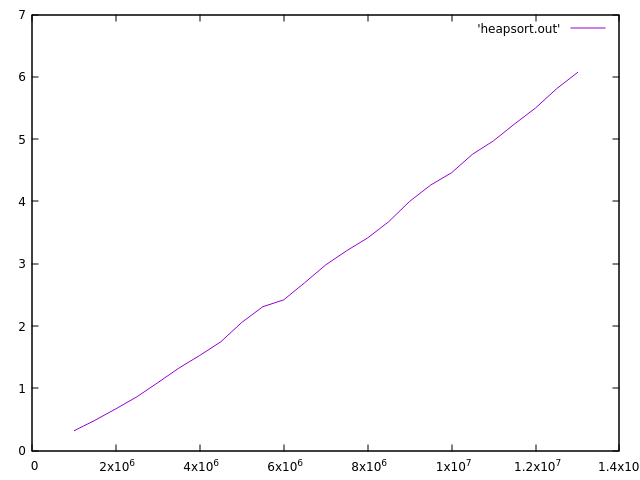
\includegraphics[scale=0.5]{empirica_heapsort.png}
\end{figure}
\end{frame}

\subsubsection{Algoritmo con eficiencia $O(2^n)$}

\begin{frame}[fragile]{Algoritmo Hanoi}
\begin{figure}[H]
\centering
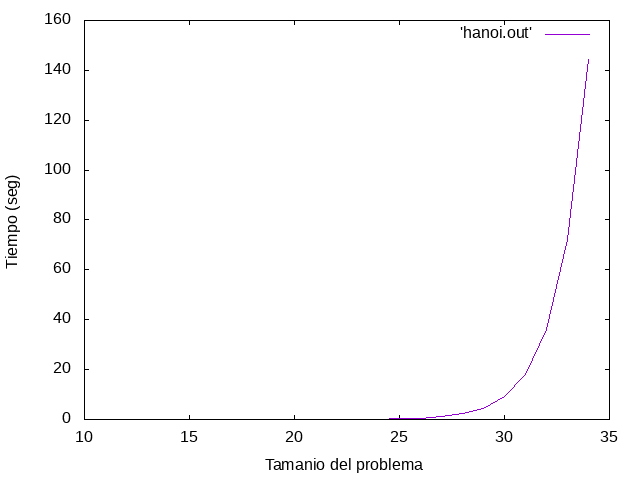
\includegraphics[scale=0.5]{empirica_hanoi.png}
\end{figure}
\end{frame}

\subsection{Variación de la eficiencia empírica}
\begin{frame}[fragile]{Variación de la eficiencia empírica}
\begin{ppio_invarianza}
La eficiencia empírica varía al cambiar de plataforma, lenguaje, etc. como mucho en una constante.
\end{ppio_invarianza}
\end{frame}

\subsection{Comparación entre algoritmos de ordenación}

\begin{frame}[fragile]{Comparación entre algoritmos de ordenación}
\begin{figure}[H]
\centering
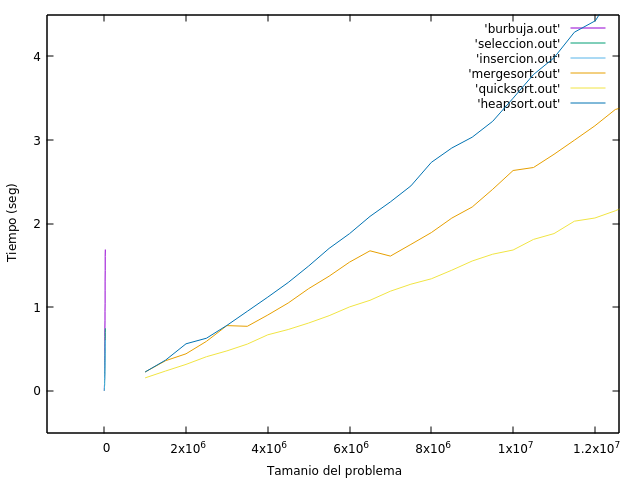
\includegraphics[scale=0.5]{empirica_ordenacion_comparacion.png}
\end{figure}
\end{frame}

\begin{frame}[fragile]{Comparación entre algoritmos de ordenación (zoom)}
\begin{figure}[H]
\centering
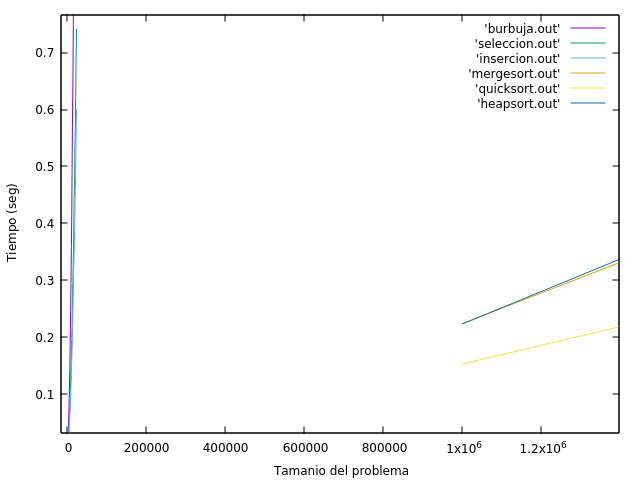
\includegraphics[scale=0.5]{empirica_ordenacion_comparacion_zoom.png}
\end{figure}
\end{frame}

\section{Cálculo de la eficiencia híbrida}

\subsection{Errores en el cálculo de la constante oculta}

\subsection{Resultados}

\subsection{Ajuste erróneo}



\begin{frame}{Blocks}
\begin{block}{Block Title}
You can also highlight sections of your presentation in a block, with it's own title
\end{block}
\begin{theorem}
There are separate environments for theorems, examples, definitions and proofs.
\end{theorem}
\begin{example}
Here is an example of an example block.
\end{example}
\end{frame}

% Placing a * after \section means it will not show in the
% outline or table of contents.



% All of the following is optional and typically not needed. 
\appendix
\section<presentation>*{\appendixname}
\subsection<presentation>*{For Further Reading}


\end{document}


